% ======================================================================
\section{Data}\label{sec:data}

This section describes how the sample was constructed, the variables used and their sources, the extent of missing data and how it is handled, and the main features of the data.

\subsection{Sample construction}

The population of interest is the set of sovereign states. It is defined as the 193 member states of the United Nations plus the State of Palestine, a UN observer state, for a total of \nNStates{} states. Countries are identified by their ISO 3166-1 alpha-3 codes, and all data sources are merged on these codes. This rules out by construction the regional and income-group aggregates that statistical databases publish alongside country data (``World'', ``Sub-Saharan Africa'', ``High income'' and so on), as well as dependent territories that are not sovereign states.

Following \citet{fanning2022}, the sample is restricted to countries with a mean population of at least \nMinPopMillion{} million over the study period. Very small states often have incomplete statistics, and some of their social and emissions data are modelled rather than measured. This leaves \nNCountries{} countries, each observed annually from \nFirstYear{} to \nLastYear{}, for a balanced grid of country-years. The period ends in \nLastYear{} because that is the last year for which the purchasing-power-parity GDP series is available for all countries.

\Cref{tab:flow} summarises how the analysis samples are derived from this population.

\begin{table}[tbp]
\centering
\small
\caption{Sample construction.}
\label{tab:flow}
\begin{tabular}{lr}
\toprule
Step & Countries \\
\midrule
UN member states and the State of Palestine & \nNStates \\
\quad with a mean population of at least \nMinPopMillion{} million, 1990--2022 & \nNCountries \\
\quad\quad with consumption-based CO$_2$ estimates (main sample) & \nNCons \\
\quad\quad with production-based CO$_2$ only & \nMissOutN \\
\midrule
Country-years 1991--2022, all \nNCountries{} countries & \nCsTotal \\
\quad classified into a configuration & \nCsClassified \\
\quad not classified: no consumption-based CO$_2$ in that year & \nCsNoCO \\
\quad not classified: social status undetermined & \nCsUndetermined \\
\bottomrule
\end{tabular}
\begin{minipage}{0.9\linewidth}\vspace{3pt}\footnotesize\textit{Notes:} Country-year counts refer to all \nNCountries{} countries in 1991--2022. The year 1990 is excluded from the classification because the ILO employment series starts in 1991. A social status is undetermined when no indicator falls short of its threshold but at least one indicator is missing (\cref{sec:methods}).\end{minipage}
\end{table}

\subsection{Social indicators}

Four social indicators define the social foundation. All come from the World Bank's World Development Indicators \citep{worldbank2024wdi}, which compile them from specialised UN agencies. Each indicator, its source and the reason for including it are described below. \Cref{tab:thresholds} in \cref{sec:methods} lists the thresholds.

\paragraph{Life expectancy at birth} (WDI series SP.DYN.LE00.IN, from the UN World Population Prospects). Life expectancy is the most widely used summary of population health. It reflects mortality at all ages and is therefore sensitive to nutrition, sanitation, health care, violence and environmental conditions. The threshold of 74 years follows \citet{fanning2022}.

\paragraph{Under-5 mortality} (SH.DYN.MORT, deaths before age five per 1{,}000 live births, from the UN Inter-agency Group for Child Mortality Estimation). Child mortality is particularly sensitive to basic services such as clean water, sanitation, vaccination and maternal care. The threshold of 25 deaths per 1{,}000 is the Sustainable Development Goal target 3.2 \citep{un2015sdg}. This indicator is not in the original doughnut thresholds. It is included because it has complete coverage and an internationally agreed target, and it complements life expectancy by focusing on the youngest age group.

\paragraph{Access to electricity} (EG.ELC.ACCS.ZS, percentage of the population with access, SDG indicator 7.1.1). Access to electricity is a basic condition for lighting, refrigeration, communication, education and modern health care. It is also the social indicator most directly connected with energy use and therefore with emissions. The threshold of 95\% follows \citet{oneill2018} and \citet{fanning2022}.

\paragraph{Employment} (100 minus SL.UEM.TOTL.ZS, the ILO modelled unemployment rate as a percentage of the labour force). Employment is a source of income and an important determinant of subjective well-being. Following both \citet{oneill2018} and \citet{fanning2022}, who describe their indicator in their supplementary information as one minus the unemployment rate from the World Development Indicators, employment is measured as the share of the labour force that is employed. The threshold is 94\%, equivalent to an unemployment rate of 6\%. Because the indicator is defined relative to the labour force rather than the whole working-age population, it does not penalise countries with low labour-force participation. It is not the employment-to-population ratio. It also does not capture informal or precarious work, underemployment or the quality of jobs, so in many low-income countries, where few people can afford to be unemployed, it overstates how well employment needs are met. It does respond to business cycles, which is why results without it are reported as a robustness check.

\paragraph{Secondary enrolment} (SE.SEC.ENRR, gross enrolment ratio, from the UNESCO Institute for Statistics) is not part of the main social foundation, although \citet{fanning2022} include it. In this panel the series covers about two thirds of country-years, with multi-year gaps for several of the largest countries. Examples are China after 2012, the United States before 2005, and Brazil and Japan before 2012--2013. A country cannot be classified as meeting the social foundation while one of its indicators is unknown (\cref{sec:methods}). Including enrolment in the main definition would therefore make classifications depend on data availability rather than on outcomes. Results with secondary enrolment added as a fifth indicator are reported as a robustness check.

\subsection{Emissions}

Emissions data come from the Global Carbon Budget 2025 \citep{friedlingstein2026}, as compiled by \citet{owid2025co2}.

\paragraph{Production-based \COtwo{}} measures fossil fuel and industrial \COtwo{} emitted within a country's territory, divided by its population. It is available for all \nNCountries{} countries in every year.

\paragraph{Consumption-based \COtwo{}} adjusts production-based emissions for trade. Emissions embodied in imported goods and services are added and those embodied in exports are subtracted. The Global Carbon Budget estimates this with a multi-regional input--output model, following the approach of \citet{peters2011}. Consumption-based estimates are available for \nNCons{} of the \nNCountries{} countries, covering \nConsPopShare\% of the sample's population in \nLastYear. They are the main emissions measure in this paper, for the reasons given in \cref{sec:literature}.

\paragraph{Total greenhouse-gas emissions including land use} (\COtwo, methane and nitrous oxide, in \COtwo-equivalents over a 100-year horizon) come from \citet{jones2023} and are used as an alternative pressure measure in the within-country models.

Both \COtwo{} series cover fossil fuels and industry and exclude emissions from land-use change. National estimates of land-use emissions are much more uncertain, and consumption-based estimates do not include them. The carbon budgets behind the boundary refer to all anthropogenic \COtwo{}, including land use. Comparing fossil and industrial emissions with the boundary therefore slightly understates overshoot for countries with net emissions from land-use change, such as countries with ongoing deforestation.

\subsection{Income}

GDP per person is measured in constant 2011 international dollars at purchasing power parity, from the Maddison Project Database 2023 \citep{bolt2025}. Purchasing-power-parity GDP adjusts for differences in price levels between countries and for inflation over time, so it is comparable across both countries and years. It is used as a control variable in the within-country models and to classify decoupling. It is available for \nNGDP{} of the \nNCountries{} countries.

\Cref{tab:data} summarises the variables, their sources and their coverage.

\begin{table}[tbp]
\centering
\small
\setlength{\tabcolsep}{3pt}
\caption{Variables, sources and coverage in the analysis panel.}
\label{tab:data}
\begin{threeparttable}
\begin{tabular}{llrrr}
\toprule
Variable & Source & Countries & Years & Coverage (\%) \\
\midrule
Life expectancy at birth & WDI (UN WPP) & 155 & 1990--2022 & 100 \\
Under-5 mortality & WDI (UN IGME) & 155 & 1990--2022 & 100 \\
Access to electricity & WDI (SDG 7.1.1) & 155 & 1990--2022 & 95 \\
Secondary gross enrolment & WDI (UNESCO UIS) & 154 & 1990--2022 & 86 \\
Employment (100 $-$ unemployment) & WDI (ILO modelled) & 155 & 1991--2022 & 97 \\
Consumption-based CO$_2$ per person & Global Carbon Budget 2025 & 114 & 1990--2022 & 73 \\
Production-based CO$_2$ per person & Global Carbon Budget 2025 & 155 & 1990--2022 & 100 \\
GHG incl.\ land use per person & \citet{jones2023} & 154 & 1990--2022 & 99 \\
GDP per person (2011 int.\$) & Maddison Project 2023 & 149 & 1990--2022 & 96 \\
\bottomrule
\end{tabular}
\begin{tablenotes}[flushleft]
\footnotesize
\item \textit{Notes:} Panel of 155 countries $\times$ 33 years. Coverage is the share of country-years with a value after interpolating interior gaps of at most 3 years. WDI: World Development Indicators.
\end{tablenotes}
\end{threeparttable}
\end{table}


\subsection{Missing data}\label{sec:missing}

\Cref{fig:coverage} shows the share of countries with an observed value for each indicator in each year. Life expectancy, under-5 mortality, production-based emissions and GDP are almost complete. Employment is complete from 1991, when the ILO modelled series begins. Access to electricity has gaps in the 1990s, when it was measured mainly through occasional household surveys. Secondary enrolment has substantial gaps throughout. Consumption-based emissions are either available for a country in every year or not at all.

\begin{figure}[tbp]
\centering
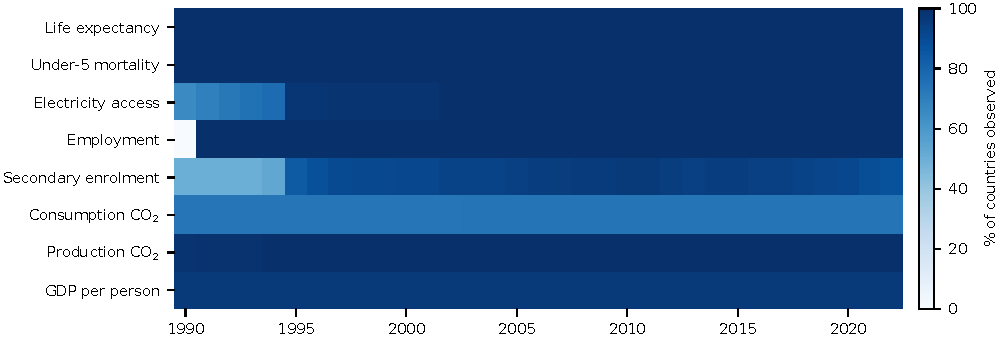
\includegraphics[width=\textwidth]{../figures/figA_coverage.pdf}
\caption{Data coverage: share of the \nNCountries{} countries with an observed value, by indicator and year, after the interpolation rules described in the text.}
\label{fig:coverage}
\end{figure}

Missing values are handled in three steps, each of which is reported and tested.
\begin{enumerate}
\item \textbf{Short interior gaps} of at most three years within a country's series are filled by linear interpolation. Gaps at the beginning or end of a series are never extrapolated. This affects \nPctInterpolated\% of all values.
\item \textbf{Electricity access} is observed only intermittently in some countries, but changes slowly. It is therefore interpolated across longer interior gaps and filled from the nearest observed year within five years at the beginning or end of the series. This adds values for \nPctFilledElectricity\% of country-years. Secondary enrolment, used only in the robustness check, is treated the same way.
\item \textbf{Classification under missing data} is asymmetric, as described in \cref{sec:methods}. A known shortfall on any observed indicator classifies a country as falling short. A country is classified as meeting the foundation only if all four indicators are observed.
\end{enumerate}

How much do the results depend on these choices? \Cref{tab:flow} shows that of the \nCsTotal{} country-years in 1991--2022, \nCsClassified{} are classified into a configuration. The rest lack consumption-based emissions (\nCsNoCO) or have an undetermined social status (\nCsUndetermined). The undetermined cases come from \nCsUndCountries, and the indicator most often missing in them is \nCsUndTopIndicator. When the entire analysis is repeated without any interpolation or gap filling, \nFillOnlyMain{} of the \nFillClassified{} classified country-years can no longer be classified, and \nFillSameShare\% of the remainder receive exactly the same configuration. The imputation rules therefore make almost no difference to the classification.

The main source of missing data is the absence of consumption-based estimates for \nMissOutN{} countries, and these countries are not a random subset. \Cref{tab:missing} compares them with the \nMissInN{} countries in the main sample, using 2011--2022 averages. The countries without consumption-based estimates are smaller (median population \nMissPopOut{} million against \nMissPopIn{} million) and poorer (median GDP per person \$\nMissGdpOut{} against \$\nMissGdpIn). They have lower life expectancy (\nMissLEOut{} against \nMissLEIn{} years) and much lower production-based emissions (\nMissProdOut~t against \nMissProdIn~t per person). \nMissOutAfrica{} of them are in Africa and \nMissOutAsia{} in Asia.

Classified with production-based emissions, \nMissOutWithin{} of these \nMissOutClassified{} countries fall short within the boundary in 2011--2022, and the number in the safe and just space is \nMissOutSafe. The main sample therefore under-represents low-emitting countries with social shortfalls. This matters for the shares of countries in each configuration, which are reported for the main sample and should be read with this in mind. It does not affect the finding that the safe and just space is empty, because none of the excluded countries is in it on the production-based measure. The robustness analysis repeats the main results with production-based emissions for all \nNCountries{} countries.

\begin{table}[tbp]
\centering
\small
\caption{Countries with and without consumption-based CO$_2$ estimates.}
\label{tab:missing}
\begin{threeparttable}
\begin{tabular}{lrrr}
\toprule
Variable (2011--2022 means) & With data (n=114) & Without (n=41) & $p$ \\
\midrule
Population (millions) & 15.0 & 7.3 & 0.013 \\
GDP per person (2011 int.\$) & 14{,}628.9 & 4{,}785.3 & 0.000 \\
Life expectancy (years) & 74.7 & 64.6 & 0.000 \\
Under-5 mortality (per 1,000) & 13.8 & 51.0 & 0.000 \\
Electricity access (\%) & 99.7 & 57.0 & 0.000 \\
Employment (\%) & 94.4 & 89.9 & 0.087 \\
Production CO$_2$ (t per person) & 3.7 & 0.7 & 0.000 \\
\bottomrule
\end{tabular}
\begin{tablenotes}[flushleft]
\footnotesize
\item \textit{Notes:} Medians across countries. $p$: two-sided Mann--Whitney test of equal distributions.
\end{tablenotes}
\end{threeparttable}
\end{table}


\subsection{Descriptive overview}

\Cref{tab:desc} reports descriptive statistics for the main sample, averaged within each of the three periods. \Cref{fig:trends} shows the median and interquartile range of each indicator across countries in every year.

\begin{table}[tbp]
\centering
\footnotesize
\setlength{\tabcolsep}{3pt}
\caption{Descriptive statistics of the consumption-based sample, period means.}
\label{tab:desc}
\begin{threeparttable}
\begin{tabular}{lrrrr}
\toprule
Variable & 1990–2000 & 2001–2010 & 2011–2022 & Min.\ N \\
\midrule
Life expectancy (years) & 69.8 [52.4, 77.3] & 72.4 [55.3, 79.9] & 74.7 [62.4, 81.8] & 114 \\
Under-5 mortality (per 1,000) & 31.1 [7.1, 148.2] & 21.6 [4.7, 104.0] & 13.8 [3.4, 58.7] & 114 \\
Electricity access (\%) & 97.1 [16.4, 100.0] & 98.4 [23.9, 100.0] & 99.7 [44.6, 100.0] & 114 \\
Employment (\%) & 93.1 [86.5, 97.5] & 93.6 [87.7, 97.2] & 94.4 [88.5, 97.3] & 114 \\
Consumption CO$_2$ (t per person) & 3.1 [0.2, 13.4] & 3.9 [0.3, 14.6] & 4.2 [0.6, 14.7] & 113 \\
Production CO$_2$ (t per person) & 2.9 [0.2, 12.2] & 3.6 [0.2, 12.1] & 3.7 [0.4, 11.8] & 114 \\
GDP per person (2011 int.\$) & 7{,}795 [1{,}370{,} 30{,}122] & 10{,}917 [1{,}786{,} 39{,}733] & 14{,}629 [2{,}631{,} 45{,}389] & 114 \\
Weakest attainment ratio & 0.77 [0.15, 1.00] & 0.94 [0.21, 1.00] & 0.96 [0.34, 1.00] & 114 \\
\bottomrule
\end{tabular}
\begin{tablenotes}[flushleft]
\footnotesize
\item \textit{Notes:} Median across countries, with the 10th and 90th percentiles in brackets. Min.\ N: the smallest number of countries with a value in any period.
\end{tablenotes}
\end{threeparttable}
\end{table}


\begin{figure}[tbp]
\centering
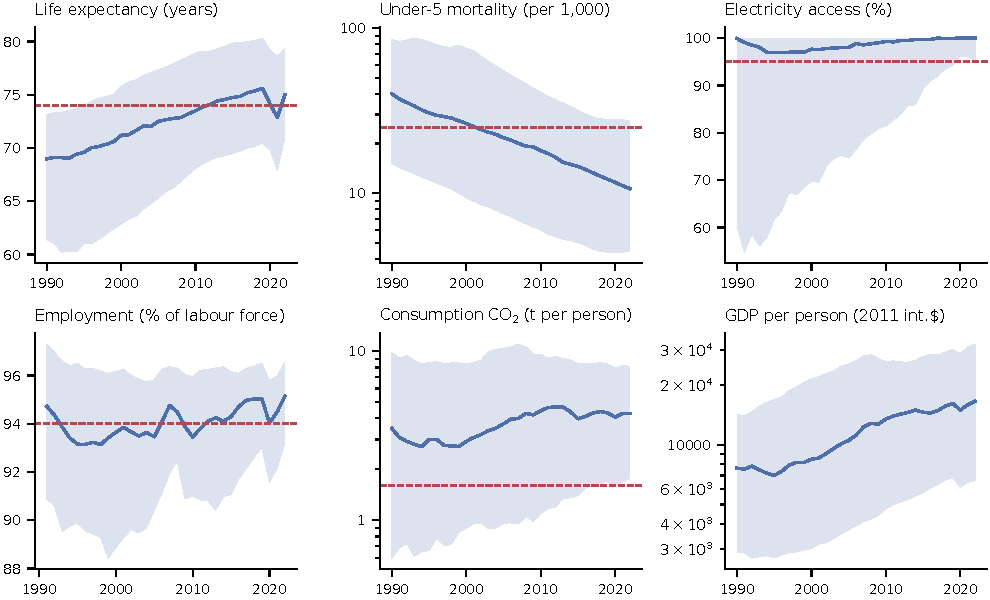
\includegraphics[width=\textwidth]{../figures/fig_trends.pdf}
\caption{Social indicators, emissions and income in the main sample, \nFirstYear--\nLastYear. Lines show the median across countries and shaded bands the interquartile range. Dashed red lines mark the social thresholds and the climate boundary.}
\label{fig:trends}
\end{figure}

Three patterns stand out. First, social outcomes improved substantially in the typical country. Median under-5 mortality fell from \nDescUFirst{} to \nDescULast{} deaths per 1{,}000 live births between 1990--2000 and 2011--2022, and median electricity access rose from \nDescElecFirst\% to \nDescElecLast\%. Second, consumption-based emissions per person in the typical country did not fall. The median rose from \nDescCOFirst~t to \nDescCOLast~t, well above the boundary throughout. Third, there is wide dispersion in every indicator, reflecting the large differences between countries in income, demography and history. Median GDP per person nearly doubled between the first and last periods, from \$\nDescGdpFirst{} to \$\nDescGdpLast.
